\vspace{10pt}

{\centering\subsection*{何锦玉:游湖南张家界}}

\addcontentsline{toc}{subsection}{何锦玉:游湖南张家界}

\renewcommand{\leftmark}{何锦玉:游湖南张家界}

\begin{figure}[htbp]

\centering

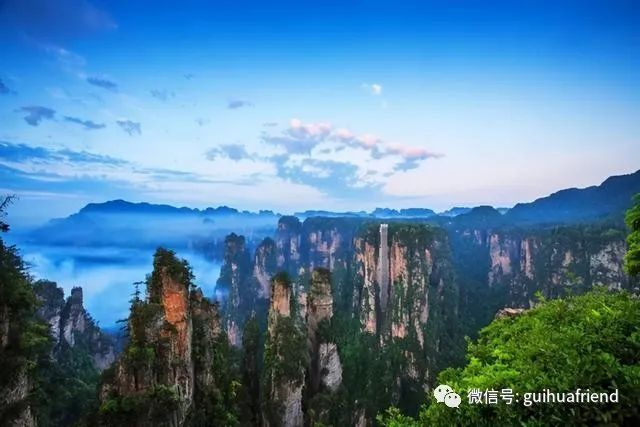
\includegraphics[width = .5\textwidth]{./ch/17.jpg}

\end{figure}



“张家界是天下第一奇山”。没错,张家界虽有形态各异的山,还有清澈见底的泉、胆大包天的猴和解不出来的迷。而且不仅有张家界,连袁家界,杨家界都有。

张家界的美在那微小的细节里。比如:垃圾桶,设计的很有创意,一组垃圾桶有两个,一个是可回收物和其他垃圾,一高一低,像那高低不平的山。垃圾桶后面有一个支架,支架上挂着垃圾桶的盖子,标出了垃圾标志。

张家界的美在那自然形成的山。在几亿年前,那里还是大海来往的通道,随着地壳运动,山被驱赶了上来。每座山都有不同的样子。“天然长城”顾名思义,就是一座接一座的山,但没有长城那么长。“金鸡独立”犹如一只鸡抬起脚爪,大声叫的样子。“食指山”,又称“一指山”,举起右手,握拳,伸出拇指,我照着样子看,有点像。

张家界的美在那顽皮的猴子。有的猴子胖的如装了一个大篮球,有的猴子瘦的只剩骨头,有的猴子没能打败猴王,被赶出猴群,有的猴子和家人一起在戏水。我拍视频时手里拿着一根黄瓜,猴子突然跑过来。我怕它因为我不给它吃,过来打我。我直接一丢,撒腿就跑。跑到一半又跑回去,没想到我随手一丢,猴子竟然接住了,大口大口的吃起来。那样子可爱极了!

张家界还有解不开的迷呢!以前土家族和苗族不分族群,可不知为何就散开了。张家界有三大古谜,至今,科学都未解开,分别是湘西赶尸、放蛊和复活咒。张家界中还有许多谜题和生物,数也数不尽,说也说不清。希望你以后去慢慢体会。







\vspace{10pt}



作者:四(1)班 何锦玉



指导老师:周瑞



投稿:2021年5月25日



发表:2021年5月25日
















                



\vspace{10pt}

\hline



